\documentclass[aps,pre,preprint]{revtex4}
% \documentclass[aps,pre,twocolumn]{revtex4-1}
% \documentclass[aps,jcp,groupedaddress,twocolumn,unsortedaddress]{revtex4}

\usepackage{amsmath}
\usepackage{amssymb}
\usepackage[dvips]{graphicx}
\usepackage{color}
\usepackage{tabularx}

\makeatletter
\makeatother

\newcommand{\recheck}[1]{{\color{red} #1}}
\renewcommand{\v}[1]{\textbf{\textit{#1}}}
\renewcommand{\d}[1]{\textsf{#1}}
% \allowdisplaybreaks

\newtheorem{theorem}{Theorem}[section]
\newtheorem{lemma}[theorem]{Lemma}
\newtheorem{proposition}[theorem]{Proposition}
\newtheorem{corollary}[theorem]{Corollary}

\newenvironment{proof}[1][Proof]{\begin{trivlist}
\item[\hskip \labelsep {\bfseries #1}]}{\end{trivlist}}
\newenvironment{definition}[1][Definition]{\begin{trivlist}
\item[\hskip \labelsep {\bfseries #1}]}{\end{trivlist}}
\newenvironment{example}[1][Example]{\begin{trivlist}
\item[\hskip \labelsep {\bfseries #1}]}{\end{trivlist}}
\newenvironment{remark}[1][Remark]{\begin{trivlist}
\item[\hskip \labelsep {\bfseries #1}]}{\end{trivlist}}

\newcommand{\qed}{\nobreak \ifvmode \relax \else
      \ifdim\lastskip<1.5em \hskip-\lastskip
      \hskip1.5em plus0em minus0.5em \fi \nobreak
      \vrule height0.75em width0.5em depth0.25em\fi}


\begin{document}

\title{The Error Estimate of Force Calculation in the Inhomogeneous Molecular Systems}
\author{Han Wang}
\affiliation{LMAM and School of Mathematical
  Sciences, Peking University}
\author{Pingwen Zhang}
% \email{pzhang@pku.edu.cn}
\affiliation{LMAM and School of Mathematical
  Sciences, Peking University}

\begin{abstract}
\end{abstract}

\maketitle

\section{Theory}

\subsection{Error estimate for
  the pairwise interactions in a charged system}

In this paper, we consider the force error, bacause the applicaions
are based on the molecular dynamics simulation.  Suppose the system is
composed by $N$ charged particles located at $\v r_1, \v r_2, \cdots,
\v r_N$ with charges $q_1, q_2, \cdots, q_N$, respectively.  We study
the force error of an arbitrary charge $i$ by calculating the
difference between the exact force and calculated force exerting on
the charge $i$, which is called the \emph{error force}
\cite{wang2012} and denoted by $\Delta \v F(\v r_i)$.
% and is denoted by
% $\Delta \v F(\v r_i) = \v F(\v r_i) - \tilde{\v F}(\v r_i)$.
The maganitude of the force computation error 
% error of the force computation
is defined by the \emph{root mean square (RMS)} \emph{error}, which is
the square root of the second moment of the error force: $\mathcal
E(\v r_i) = \sqrt{\langle\vert\Delta\v F(\v r_i)\vert^2\rangle}$.  The
notation $\langle\cdot\rangle$ means ensemble average.  We also
estimate the the ensemble average of the error force (also called
\emph{mean error force}), namly $\langle\Delta\v F(\v r_i)\rangle$,
which plays an important role in the error analysis of the
short-range inhomogeneous systems~\cite{wang2012}.

One of the main results of this research is the error estimate for
the error force that can be written as a summation of
pairwise interactions:
\begin{theorem}\label{thm:tmp1}
  Let a periodic molecular system be composed by $N$ charged particles
  located at $\v r_1, \v r_2, \cdots, \v r_N$ with charges $q_1, q_2,
  \cdots, q_N$, respectively.
  % Let the box vectors be $\v a_\alpha, \
  % \alpha=1,2,3$, and denote the lattice in the real space by $\v n =
  % n_1 \v a_1 + n_2 \v a_2 + n_3 \v a_3$, $n_\alpha\in\mathbb Z$.
  If the error force of an arbitary particle $i$ is
  \begin{align}\label{eqn:thm-error-force}
    \Delta \v F(\v r_i) =
    % \sum^\ast_{\v n}
    \sum_{j=1}^N\,q_iq_j \v K(\v r_i - \v r_j),
  \end{align}
  then the mean error force is
  \begin{align}\label{eqn:thm-meanf}
    \langle\Delta\v F(\v r_i)\rangle
    =q_i\, [\v K\ast\rho_q](\v r_i),
  \end{align}
  and the RMS error is
  \begin{align}\nonumber
    \mathcal E (\v r_i) 
    = &\,
    q_i^2\,[(\v K)^2\ast\rho_{q^2}] (\v r_i) + 
    q_i^2\,[\v K\ast\rho_{q}]^2 (\v r_i) \\\label{eqn:thm-error}
    &+
    q_i^2\,\int_{\mathbb R^3\times\mathbb R^3}
    \v K(\v r_i-\v r')\cdot
    \v K(\v r_i-\v r'')\,
    C_{q^2}(\v r', \v r'')\,
    \d d\v r'\d d\v r''.
  \end{align}
  Where $\ast$ denotes the convolution, and
  % The $\rho_q$, $\rho_{q^2}$ and
  % $C_{q^2}$ are defined by:
  \begin{align}\label{eqn:def-rhoq}
    \rho_q(\v r)
    &= 
    \bigg\langle
    \sum_{j = 1}^N
    \,q_j\,\delta(\v r - \v r_j)
    \bigg\rangle,\\\label{eqn:def-rhoq2}
    \rho_{q^2}(\v r)
    &= 
    \bigg\langle
    \sum_{j = 1}^N
    \,q^2_j\,\delta(\v r - \v r_j)
    \bigg\rangle,\\\label{eqn:def-rho2}
    \rho^{(2)}(\v r, \v r')
    &= 
    \bigg\langle
    \sum_{j\neq k}
    q_jq_k\delta(\v r-\v r_j)\delta(\v r'-\v r_k)
    \bigg\rangle,\\\label{eqn:def-c}
    C(\v r, \v r')
    &=
    \rho^{(2)}(\v r, \v r')    
    - \rho_q(\v r)\rho_q(\v r').
  \end{align}
  Notice the definitions of $\rho_q(\v r)$, $\rho_{q^2}(\v r)$ and
  $\rho^{(2)}(\v r, \v r')$ are periodically extended to
  $\mathbb{R}^3$, $\mathbb{R}^3$ and $\mathbb{R}^3\times\mathbb R^3$,
  respectively.
\end{theorem}
\begin{proof}
  By definition, the mean error force is:
  \begin{align*}
    \langle\Delta\v F(\v r_i)\rangle
    &=
    q_i\bigg\langle \sum_{j=1}^Nq_j\v K(\v r_i -\v r_j)\bigg\rangle\\
    &=
    q_i\int_{\mathbb R^3}\v K(\v r_i - \v r')
    \bigg\langle \sum_{j=1}^Nq_j\delta (\v r' -\v r_j)\bigg\rangle
    \,\d d\v r'\\
    &= 
    q_i\, [\v K\ast\rho_q](\v r_i),
  \end{align*}
  The RMS force error is calculated by:
  \begin{align} \nonumber
    \langle\vert\Delta\v F(\v r_i)\vert^2\rangle
    =\,&
    q_i^2\bigg\langle\sum_{j,k}
    q_jq_k\v K(\v r_i - \v r_j)\cdot\v K(\v r_i - \v r_k)\bigg\rangle \\ \nonumber
    =\,&
    q_i^2\bigg\langle\sum_{j=1}^N
    q_j^2\vert\v K(\v r - \v r_j)\vert^2
    \bigg\rangle +
    q_i^2\bigg\langle\sum_{j\neq k}
    q_jq_k \v K(\v r - \v r_j)\cdot\v K(\v r - \v r_k)
    \bigg\rangle \\ \nonumber
    =\,&
    q_i^2\int_{\mathbb R^3}
    \vert\v K(\v r_i - \v r')\vert^2\rho_{q^2}(\v r')\,\d d\v r'
    \\\label{eqn:prf-error-step3}
    & +
    q_i^2\int_{\mathbb R^3\times\mathbb R^3}
    \v K(\v r_i - \v r')\cdot\v K(\v r_i - \v r'')\,
    \rho^{(2)}(\v r', \v r'')
    \,\d d\v r'\d d\v r''\\\nonumber
    =\,&
    q_i^2\int_{\mathbb R^3}
    \vert\v K(\v r_i - \v r')\vert^2\rho_{q^2}(\v r')\,\d d\v r'
    +
    q_i^2
    \bigg[
    \int_{\mathbb R^3}
    \v K(\v r_i - \v r')\rho_{q}(\v r')\,\d d\v r'
    \bigg]^2
    \\ \nonumber
    & +
    q_i^2\int_{\mathbb R^3\times\mathbb R^3}
    \v K(\v r_i - \v r')\cdot\v K(\v r_i - \v r'')\,
    C(\v r', \v r'')
    \,\d d\v r'\d d\v r''.\qquad\qed
    % = \,&
    % q_i^2\,[(\v K)^2\ast\rho_{q^2}] (\v r_i) + 
    % q_i^2\,[\v K\ast\rho_{q}]^2 (\v r_i) \\
    % &+
    % q_i^2\,\int_{\mathbb R^3\times\mathbb R^3}
    % \v K(\v r_i-\v r')\cdot
    % \v K(\v r_i-\v r'')\,
    % C_{q^2}(\v r', \v r'')\,
    % \d d\v r'\d d\v r''. \qquad\qed
    % \int_{\mathbb R^3\times\mathbb R^3}\v K(\v r - \v r')\cdot\v K(\v r - \v r'')\rho(\v r', \v r'')\,\d d\v r'\d d\v r''.
  \end{align}
\end{proof}
Here are some remarks concerning Theorem~\ref{thm:tmp1}:
\begin{itemize}
% \item
%   This theorem provides the error estimate for the interactions, whose
%   error force can be
%   written as a summation of pairwise interactions. 
  % It should be well defined for $\v r = \v 0$. For
  % the cut-off method, $\v K(\v 0) = \v 0$. For the reciprocal part 
\item The densities $\rho_q(\v r)$ and $\rho_{q^2}(\v r)$ defined in
  Eqn.~\eqref{eqn:def-rhoq} and \eqref{eqn:def-rhoq2} are called \emph{the
    first order charge distribution} and \emph{the
    second order charge distribution},
  respectively.
  $\rho^{(2)}(\v r, \v r')$ in Eqn.~\eqref{eqn:def-rho2}
  is the \emph{pairwise charge distribution}.
  When the positions of any two different charges are independent,
  $\rho^{(2)}(\v r, \v r') = \frac{N-1}{N}\rho_q(\v r)\rho_q(\v r')$.
  Since $N$ is always a large number in real simulations, we take
  $\rho^{(2)}(\v r, \v r') = \rho_q(\v r)\rho_q(\v r')$ for convenience.
  $C_{q^2}(\v r, \v r')$ defined in
  Eqn.~\eqref{eqn:def-c} is the \emph{pairwise charge correlation function},
  which describes the strength of the correlation between  two
  different charges. When they are independent, $C_{q^2}(\v r, \v r')$
  vanishes, otherwise $C_{q^2}(\v r, \v r') \neq 0$.
  Most of the error estimates assumed the independency of the
  particles in the system~\cite{kolafa1992cutoff, deserno1998mue2, wang2010optimizing, wang2012},
  however, this could be problematic in the strongly correlated
  systems~\cite{deserno1998mue2, wang2010optimizing}.
  Also see Sec.~\ref{sec:example3} for example.
\item
  The \emph{pairwise form}
  of the interaction (see Eqn.~\eqref{eqn:thm-error-force}) is the key to derive
  the error estimates Eqn.~\eqref{eqn:thm-meanf} and \eqref{eqn:thm-error}.
  The function $\v K(\v r)$ is called \emph{the error force
    kernel}.
  By setting $q_i = q_j = 1$, the theorem~\ref{thm:tmp1} directly proves
  the error estimates for the short-range interaction
  in inhomogeneous systems, which was derived in Ref.~\cite{wang2012}. 
\item Analog to the short-range error estimate~\cite{wang2012}, the
  three terms on the r.h.s. of Eqn.~\eqref{eqn:thm-error} are called the
  homogeneity error, the inhomogeneity error and the correlation
  error, respectively.
  This is denoted by:
  \begin{align}\label{eqn:error-split}
    \langle\vert\Delta\v F(\v r_i)\vert^2\rangle
    =
    \mathcal E^2_{\textrm{homo}}(\v r_i) +
    \mathcal E^2_{\textrm{inhomo}}(\v r_i) +
    \mathcal E_{\textrm{correlation}}(\v r_i).
  \end{align}
  The homogeneity error and the inhomogeneity
  error can be calculated at the cost of $\mathcal O(N\log N)$ by the
  fast Fourier transform (FFT) (see Ref.~\cite{wang2012} for details).
  However, the full calculation of the correlation error costs $\mathcal
  O(N^2\log N)$, because it involves a twofold convolution.
  % In this
  % study, the contribution of the correlation error is neglicted.
  % In
  % section~\ref{sec:tmp3}, it is shown neglicting the 
\item A non-varnishing mean error force~\eqref{eqn:thm-meanf} was proved
  to be
  harmful to the calculation of the short-range interaction
  in inhomogeneity systems~\cite{wang2012}.
  In the case of the charged system, this
  term is non-zero only when the system is NOT locally neutral,
  i.e. a non-zero first order charge distribution. For
  most of the simulation cases, the locally neutral condition is
  satisfied, so the mean error force and the inhomogeneity error
  vanish.
  % The
  % serious artifical effect due to the inhomogeneity error of
  % short-range interaction~\cite{wang2012} does not exist in most
  % charged systems.
\end{itemize}

\subsection{First neighbor approximation of the correlation
error}

In this section, we consider the first neighbor approximation of the
correlation error. Here ``first neighbors'' means the neighboring
atoms that are connected by the chemical bond.  In most molecular
force fields, such bonds are modeled by a rigid connection between two
atoms.  Therefore, the correlation between such an atom pair is very
strong. As an example, we consider a typical three point charge water
model TIP3P~\cite{jorgensen1983comparison}: each hydrogen atom carries
a charge of $q_{\textrm{H}} = +0.417e$ and each oxygen atom carries a charge of
$q_{\textrm{O}} = -0.834e$. Within one molecule, the H-O bond and H-O-H angle are
rigid. 
% In the system of water, the relative position of the oxygen and
% hydrogen atoms within one molecule is fixed. Therefore, according
% to this property, it is possible to improve the quality of the
% error estimate.
Starts from Eqn.~\eqref{eqn:prf-error-step3},
\begin{align} \nonumber
  \langle\vert\Delta\v F(\v r_i)\vert^2\rangle
  =\,&
  q_i^2\int_{\mathbb R^3}
  \vert\v K(\v r_i - \v r')\vert^2\rho_{q^2}(\v r')\,\d d\v r'
  \\
  & +
  q_i^2\int_{\mathbb R^3\times\mathbb R^3}
  \v K(\v r_i - \v r')\cdot\v K(\v r_i - \v r'')\,
  \rho^{(2)}(\v r', \v r'')
  \,\d d\v r'\d d\v r'',
\end{align}
where the definition of $\rho^{(2)}(\v r', \v r'')$ is given by
Eqn.~\eqref{eqn:def-rho2}.
% \begin{align}
%   q_{q^2}(\v r', \v r'') =
%   \bigg\langle
%   \sum_{j\neq k}q_j q_k\delta(\v r' - \v r_j)\delta(\v r'' - \v r_k)
%   \bigg\rangle.
% \end{align}
We seperately consider the first neighbor contribution
and other contributions to
the pairwise density $\rho^{(2)}(\v r', \v r'')$.  Denoting
$\Omega_j = \{ \,k\,\vert\,
\textrm{atom $k$ is the first neighbor of atom $j$} \,\}$,
% the set of the first neighbors of the $j$-th atom by $\Omega_j$,
we have:
\begin{align}\label{eqn:split-rho-q2}
  \rho^{(2)}(\v r', \v r'')
  = &\,
  \bigg\langle
  \sum_j\sum_{k\in\Omega_j}q_j q_k\delta(\v r' - \v r_j)\delta(\v r'' - \v r_k)
  \bigg\rangle
  +
  \bigg\langle
  \sum_j\sum_{k\notin\Omega_j}q_j q_k\delta(\v r' - \v r_j)\delta(\v r'' - \v r_k)
  \bigg\rangle.
\end{align}
For any atom $k$ that is not the first neighbor of atom $j$, we
assume that its position is independent with atom $j$, then
second part on the r.h.s. of the Eqn.~\eqref{eqn:split-rho-q2} is
approximately $\frac{N-3}{N}\rho_q(\v r')\rho_q(\v r'')\approx
\rho_q(\v r')\rho_q(\v r'')$.
% If the number of atoms in the system is
% large, this should be a good approximation.
Therefore, the first part
on the r.h.s. of Eqn.~\eqref{eqn:split-rho-q2} is actually the
pairwise charge corrlation function:
\begin{align}\label{eqn:fnc-correlation-water}
  C_{q^2}(\v r', \v r'') =
  \bigg\langle
  \sum_j\sum_{k\in\Omega_j}q_jq_k\delta(\v r' - \v r_j)\delta(\v r'' - \v r_k)
  \bigg\rangle.
\end{align}
% If connected by the chemical bond, the position of the first neighbors
% $k$ is not independent with the atom $j$, so their correlation is
% strong, and should be calculated explicitly to improve the quality of
% the error estimate.
By inserting Eqn.~\eqref{eqn:fnc-correlation-water} into
the correlation error, we have:
\begin{align}
  \mathcal E_{\textrm{correlation}}(\v r_i)
  = q_i^2\sum_j\sum_{k\in\Omega_j}q_jq_k
  \big\langle
  \v K(\v r_i - \v r_j)\cdot\v K(\v r_i - \v r_k)
  \big\rangle_{\v r_j,\v r_k}
\end{align}
Denoting the index set of the oxygen atoms by $\Omega_{\textrm{O}}$,
and the index set of the hydrogen atoms by $\Omega_{\textrm{H}}$, 
we have:
\begin{align}\nonumber
  \mathcal E_{\textrm{correlation}}(\v r_i)
  = &\,
  q_i^2\sum_{j\in\Omega_{\textrm{O}}}\sum_{k\in\Omega_j}q_jq_k
  \big\langle
  \v K(\v r_i - \v r_j)\cdot\v K(\v r_i - \v r_k)
  \big\rangle_{\v r_j,\v r_k} \\ \nonumber
  &\,+ 
  q_i^2\sum_{j\in\Omega_{\textrm{H}}}\sum_{k\in\Omega_j}q_jq_k
  \big\langle
  \v K(\v r_i - \v r_j)\cdot\v K(\v r_i - \v r_k)
  \big\rangle_{\v r_j,\v r_k} \\\nonumber
  = &\,
  q_i^2
  \int_{\mathbb R^3}
  \v K(\v r_i - \v r')\cdot
  \big\langle
  q_{\textrm{H}}\v K(\v r_i - \v r' + \v s_{\textrm{H}_1})+
  q_{\textrm{H}}\v K(\v r_i - \v r' + \v s_{\textrm{H}_2})
  \big\rangle\,\rho_{\textrm{O}}(\v r')
  \d d\v r' \\\label{eqn:c-error-1}
  & \,+
  q_i^2
  \int_{\mathbb R^3}
  \v K(\v r_i - \v r')\cdot
  \big\langle
  q_{\textrm{O}}\v K(\v r_i - \v r' + \v s_{\textrm{O}})+
  q_{\textrm{H}}\v K(\v r_i - \v r' + \v s_{\textrm{H}})
  \big\rangle\,\rho_{\textrm{H}}(\v r')
  \d d\v r'
\end{align}
If positions of the three atom within one molecule are
$\v r_{\textrm{H}_1}$, $\v r_{\textrm{H}_2}$ and $\v r_{\textrm{O}}$, then
$\v s_{\textrm{H}_1} = \v r_{\textrm{H}_1} - \v r_{\textrm{O}}$, 
$\v s_{\textrm{H}_2} = \v r_{\textrm{H}_2} - \v r_{\textrm{O}}$,
$\v s_{\textrm{O}} = \v r_{\textrm{O}} - \v r_{\textrm{H}_1}$ and
$\v s_{\textrm{H}} = \v r_{\textrm{H}_2} - \v r_{\textrm{H}_1}$.
The two ensemble averages in Eqn.~\eqref{eqn:c-error-1}
is taken over all possible water directions 
at position $\v r'$. As an approximation, we
assume these averages are  spacially uniform, namely independet with $\v r'$.
This assumption may be  problematic
in the regions where the preference of water  drection is different
with others.
% In the example considered by the present paper in section~\ref{sec:tmp3},
% it is shown to be a good approximation to obtain the estimate of the
% correlation error.
One possible way to calculate the ensemble averages in
Eqn.~\eqref{eqn:c-error-1} is by the Fourier transform
of the error force kernel:
\begin{align} \nonumber
  &\big\langle
  q_{\textrm{H}}\v K(\v r_i - \v r' + \v s_{\textrm{H}_1})+
  q_{\textrm{H}}\v K(\v r_i - \v r' + \v s_{\textrm{H}_2})
  \big\rangle \\ \nonumber
  =\,&
  \frac1V\bigg\langle
  \sum_{\v m}
  q_{\textrm{H}}\hat{\v K}(\v m)
  e^{2\pi i\v m\cdot(\v r_i - \v r' + \v s_{\textrm{H}_1})} +
  \sum_{\v m}
  q_{\textrm{H}}\hat{\v K}(\v m)
  e^{2\pi i\v m\cdot(\v r_i - \v r' + \v s_{\textrm{H}_2})}
  \bigg\rangle \\\nonumber
  =\,&
  \frac1V\sum_{\v m}
  \hat{\v K}(\v m)
  e^{2\pi i\v m\cdot(\v r_i - \v r')}
  \,  
  \langle
  q_{\textrm{H}}\,e^{2\pi i\v m\cdot\v s_{\textrm{H}_1}} +
  q_{\textrm{H}}\,e^{2\pi i\v m\cdot\v s_{\textrm{H}_2}}
  \rangle,
\end{align}
where ``$\wedge$'' denotes the forward Fourier transform. By denoting
\begin{align}
  \hat T_{\textrm{O}}(\v m)
  &= 
  \langle
  q_{\textrm{H}}\,e^{2\pi i\v m\cdot\v s_{\textrm{H}_1}} +
  q_{\textrm{H}}\,e^{2\pi i\v m\cdot\v s_{\textrm{H}_2}}
  \rangle,\\
  \hat T_{\textrm{H}}(\v m)
  &= 
  \langle
  q_{\textrm{O}}\,e^{2\pi i\v m\cdot\v s_{\textrm{O}}} +
  q_{\textrm{H}}\,e^{2\pi i\v m\cdot\v s_{\textrm{H}}}
  \rangle.
\end{align}
The Eqn.~\eqref{eqn:c-error-1} becomes:
\begin{align}\nonumber
  \mathcal E_{\textrm{correlation}}(\v r_i)
  =&\,
  q_i^2
  \int_{\mathbb R^3}
  \v K(\v r_i - \v r')\cdot
  (\hat T_{\textrm{O}}\hat{\v K})^{\vee}(\v r_i - \v r')
  \,\rho_{\textrm{O}}(\v r')
  \,\d d\v r' \\\label{eqn:c-error-water}
  & \,+
  q_i^2
  \int_{\mathbb R^3}
  \v K(\v r_i - \v r')\cdot
  (\hat T_{\textrm{H}}\hat{\v K})^{\vee}(\v r_i - \v r')
  \,\rho_{\textrm{H}}(\v r')
  \,\d d\v r',
\end{align}
where ``$\vee$'' denotes the backward Fourier transform.
In the Fourier space, the error force kernel $\v K(\v r)$ is
influenced by the prefactors $T_{\textrm{O}}$ and $T_{\textrm{H}}$,
which are accounting for the atomic correlation within one water
molecule.

% For the second term, do variable change $\v r'' = \v r' + \v s$, we have:
% \begin{align}
%   \textrm{II} = & 
%   q_i^2
%   \int_{\mathbb R^3}\d d\v r'\v K(\v r_i - \v r')
%   \int_{\mathbb R^3}\d d\v s\,
%   \v K(\v r_i - \v r' - \v s)\,
%   \rho_{q^2}(\v r', \v r' + \v s).
% \end{align}
% Split the integral region of the variable $\v s$ into the first
% neighbor shell $\mathcal B(\v r', R_s)$ and the reset $\mathbb R -
% \mathcal B(\v r', R_s)$. In the case of water, the first neighbor
% shell means the region where a single molecule occupies. Within this
% shell, the relative position of the oxygen and two hydrogens are
% always fixed. Outside of the first neighbor shell, the position of
% oxygens and hydrogens are belongs to different molecules, so the their
% positions are assumed to be independent. In most cases, the first
% neighbor shell is small comparing to the simulation box size,
% therefore,
% \begin{align}\nonumber
%   \textrm{II}_{\textrm{out}} = & \,
%   q_i^2
%   \int_{\mathbb R^3}\d d\v r'\v K(\v r_i - \v r')
%   \int_{\mathbb R^3 - \mathcal B(\v r', s)}\d d\v s\,
%   \v K(\v r_i - \v r' - \v s)\,
%   \rho_{q^2}(\v r', \v r' + \v s) \\ \nonumber
%   = &\,
%   q_i^2
%   \int_{\mathbb R^3}\d d\v r'\v K(\v r_i - \v r') \rho_q(\v r')
%   \int_{\mathbb R^3 - \mathcal B(\v r', s)}\d d\v s\,
%   \v K(\v r_i - \v r' - \v s)\,
%   \rho_q(\v r' + \v s) \\
%   \approx &\,
%   q_i^2
%   [\v K\ast\rho_{q}]^2 (\v r_i)
% \end{align}



\subsection{Ewald summation and its error estimate}
The Ewald method divides the electrostatic interaction in to three
parts: the direct part, the reciprocal part and the correction
part:
\begin{equation}
E = E_{\textrm{dir}} + E_{\textrm{rec}} + E_{\textrm{corr}},
\end{equation}
where 
\begin {align}\label{eqn:tmp2}
E_{\textrm{dir}} & = \frac12 \sum^{\ast}_{\v n}
\sum_{i,j = 1}^{N} \frac{q_iq_j \textrm{erfc}(\beta \vert\v{r}_{ij} + \v{n}\vert)}
{\vert\v{r}_{ij} + \v{n}\vert} \\\label{eqn:tmp3}
E_{\textrm{rec}} & = \frac1{2\pi V} \sum_{\v m \neq 0}
\frac{\exp(-\pi^2\v m^2 / \beta^2)}{\v m^2} S(\v m) S(-\v m) \\\label{eqn:tmp4}
 E_{\textrm{corr}}& = -\frac\beta{\sqrt \pi} \sum_{i=1}^N q_i^2
\end {align}
The distance between the two particles is denoted by $\v r_{ij} = \v
r_i - \v r_j$.  The lattice in the real space is denoted
by $\v n = n_1 \v a_1 + n_2 \v a_2 + n_3 \v a_3$, where $\v a_\alpha,
\ \alpha=1,2,3$ are box vectors. the structure factor $S(\v m)$ is
defined by
\begin{equation}\label{sm1}
S(\v m) = \sum_{j=1}^N q_j \exp (2 \pi i \v m \cdot \v r_j),
\end{equation}
where $\v m = m_1 \v a_1^\ast + m_2 \v a_2^\ast + m_3 \v a_3^\ast$ is
the reciprocal space lattice vectors. $\v a_\alpha^\ast,\ \alpha = 1,
2, 3$ are conjugate reciprocal vectors of $\v a_\alpha$, defined by
$\v a_\alpha \cdot \v a_\beta^\ast = \delta_{\alpha\beta}$. and $V =
\v a_1 \cdot \v a_2 \times \v a_3$ is the volume of the box.

The complementary error function $\textrm{erfc}(r)$ in
Eqn.~\eqref{eqn:tmp2} decays exponentially as $r$ goes to infinity.
Therefore, it is a short-range interaction in the real space, which
can be calculated by the standard cut-off and neighbor list
method~\cite{frenkel02b} at a cost of $\mathcal O(N)$.  The reciprocal
part also decays exponentially as the maganitude of the Fourier mode
$\vert\v m\vert$ increases. Therefore, in practice, the infinit
summation in Eqn.~\eqref{eqn:tmp3} is truncated, and only a finite
summation is calculated:
% Both the direct and the reciprocal parts are calculated by cut-off in
% real and reciprocal space, respectively.
% For the reciprocal part the cut-offed energy reads
\begin{align}\label{eqn:tmp6}
  E^{\textrm{tr}}_{\textrm{rec}} & =
  % \frac1{2\pi V}
  \sum_{
    \begin{subarray}{c}
      \vert m_\alpha\vert < K_\alpha/2\\
      \v m\neq 0
    \end{subarray}}
  % \frac{\exp(-\pi^2\v m^2 / \beta^2)}{\v m^2} S(\v m) S(-\v m)   
  f(\v m)\, S(\v m) S(-\v m),
\end{align}
where, for short,
\begin{align}
  f(\v m) := \frac{\exp(-\pi^2 \v m^2 / \beta^2)}{2\pi V \v m^2},
\end{align}
and $K_\alpha$ is the number of Fourier modes used on direction
$\alpha$.  The truncated reciprocal force acting on particle $i$ is
\begin{align}\nonumber
  \v F^{\textrm{tr}}_{\textrm{rec}}(\v r_i)
  &= 
  q_i 
  \sum_{
    \begin{subarray}{c}
      \vert m_\alpha\vert < K_\alpha/2\\
      \v m\neq 0
    \end{subarray}}
  \v g(\v m) \,
  S(-\v m)\,
  e^{2\pi i\v m\cdot\v r_i}, \\\label{eqn:tmp8}
  &= 
  \sum_j   q_iq_j
  \sum_{
    \begin{subarray}{c}
      \vert m_\alpha\vert < K_\alpha/2\\
      \v m\neq 0
    \end{subarray}}
  \v g(\v m) \,
  e^{2\pi i\v m\cdot\v r_{ij}},
\end{align}
where
\begin{align}
  \v g(\v m) = -4 \pi \v m i f(\v m).
\end{align}


% Ref.~\cite{wang2010optimizing} pointed out that it is reasonable and
% convenient to estimate the error for the direct and reciprocal part
% seperately, namely $\Delta\v F(\v r_i) = \Delta\v F_{\textrm{dir}}(\v
% r_i) + \Delta\v F^{\textrm{tr}}_{\textrm{rec}}(\v r_i)$.  The
% $\Delta\v F_{\textrm{dir}}$ and $ \Delta\v
% F^{\textrm{tr}}_{\textrm{rec}}$ denote the direct error force and
% reciprocal error force, respectively.  The superscript ``tr'' denotes
% the reciprocal force is calculated by truncating the infinite Ewald
% summation. Other superscripts are introduced later in the paper to
% denote the error force of the fast algoritms
% that treat the Ewald summation more elaborately.

Both the direct part and reciprocal part of the Ewald summation can be
written in the pairwise form of Eqn.~\eqref{eqn:thm-error-force}.  The direct
error force kernel is defined by:
% The direct part is a short-range interaction in real space, so it is
% usually treated by the cut-off method, which gives a error force
% kernel of
\begin{align}
  \v K^{\textrm{cut}}_{\textrm{dir}}(\v r) =
  \left\{
    \begin{aligned}
      &\,0, &\quad & r \leq r_c;\\
      &
      \Big[
      \frac{2\beta}{\sqrt\pi} e^{-\beta^2r^2} + \frac{\textrm{erfc}(\beta r)}{r}
      \Big]\frac{\v r}{r^2}
      ,& & r > r_c,
      % \frac{\textrm{erfc}(\beta\vert\v r\vert)}{\vert\v r\vert}
    \end{aligned}
  \right.
\end{align}
where $r = \vert\v r\vert$, and $r_c$ is the cut-off radius in the
real space.
% The reciprocal error force, namely the difference between
% the the exact and truncated reciprocal force, is
% \begin{align}
%   \Delta \v F^{\textrm{tr}}_{\textrm{rec}}(\v r_i)
%   = & - 
%   \sum_j\,q_iq_j
%   \sum_{\vert m_\alpha\vert \geq K_\alpha/2}
%   \v g(\v m) \,
%   e^{2\pi i\v m\cdot\v r_{ij}}.
% \end{align}
% Therefore,
The reciprocal error force kernel is given by:
\begin{align}
  \v K^{\textrm{tr}}_{\textrm{rec}}(\v r) =
  \sum_{
      \vert m_\alpha\vert \geq K_\alpha/2}
  \v g(\v m) \,
  e^{2\pi i\v m\cdot\v r}.
\end{align}
By the Therefore \ref{thm:tmp1}, the error estimate of the
truncated Ewald summation is straightforward.


% Ref. \cite{short} pointed out that the inhomogeneity error is more
% harmful than the homogeneity error, so it is interesting to analyze
% the inhomogeneity error. Apply the Fourier transform on both sides of
% Eqn. \eqref{eqn:tmp10} and \eqref{eqn:tmp18}:
% \begin{align}  
%   \langle\Delta\v F_{\textrm{dir}}\rangle^\wedge(\v m)
%   &= q_i\,\hat{\v K}^c_{\textrm{dir}}(\v m)\cdot\hat\rho_q(\v m)\\
%   \langle\Delta\v F_{\textrm{rec}}\rangle^\wedge(\v m)
%   &= -q_i\,\hat{\v K}^c_{\textrm{rec}}(\v m)\cdot\hat\rho_q(\v m)
% \end{align}
% If the charge distribution is \emph{locally} neutral, then all modes
% of the first order density distribution vanishes, and $\langle\Delta\v
% F_{\textrm{dir}}\rangle = \langle\Delta\v F_{\textrm{rec}}\rangle = 0$.




\subsection{The smooth particle mesh Ewald method \&
the staggered mesh Ewald method}

The naive calculation of the reciprocal Ewald summation
\eqref{eqn:tmp6} will result in a computational cost of $\mathcal
O(N^2)$. It has been shown that with a careful tuning of parameter
$\beta$, real space cut-off radius $r_c$
and the reciprocal space truncation $K_\alpha$, the
optimal computational cost is $\mathcal O(N^{3/2})$~\cite{perram1988asc},
which becomes not applicable when the system
size is larger than several hundreds of charged particles. Both the
particle mesh Ewald (PME) \cite{darden1993pme} and the smooth particle
mesh Ewald (SPME) \cite{essmann1995spm} methods are designed to reduce
the computational cost to $\mathcal O(N\log N)$ in nearly the same
way.  Since the SPME method is more precise \cite{deserno1998mue1} and
more popular than the PME, we will focus our discussion on the
former. All the error estimates develop by the current paper can be
easily extended to the PME method.  The principle idea of the SPME method
is first to calculate the term $e^{2\pi i\v m\cdot\v r}$ on a uniform
lattice in the real space.  Therefore, all Fourier transforms can be
accerlerated by the fast Fourier transform (FFT) algoritm, that is why the
computational cost of SPME is reduced to $\mathcal O(N\log N)$. Then,
for any particle position $\v r_i$, the value of $e^{2\pi i\v m\cdot\v
  r_i}$ is interpolated by the known values on the neighboring lattice
points.  The PME method uses Lagrangian interpolation, while the SPME
uses B-spline interpolation,  which is more precise, and has higher order
of smoothness.

The SPME method provides two possibilities of calculating the
reciprocal force. The first one is to differentiate (with respect to
the particle position) the reciprocal term of the truncated Ewald
energy and then approximate the derived force \eqref{eqn:tmp8} by the
B-spline interplation. This way is called
\emph{ik--differentiation}~\cite{deserno1998mue1}.
The alternative way notices the high-order
smoothness of the B-spline interpolation, and derive the force by
differentiating the B-spline approximated reciprocal Ewald energy
(also truncated). The second way was proposed by the original SPME paper
\cite{essmann1995spm}, and is called the \emph{analytical
  differentiation}~\cite{deserno1998mue1}.
It has been shown that using the same parameters,
the ik-differentiation is more precise than the analytical
differentiation, but it requres twice more FFTs, which is a bottleneck
for the communication in parallel
implementations~\cite{wang2010optimizing}.
For the ik-differentiation, the calculated force is not the negative
gradient of the calculated energy. The analytical differentiation
does not have this problem, but it (to the approximation precision)
violates the Newton's third law.
Since the SPME method is
not the point of the present paper, we refer the readers to, for
example, Ref. \cite{essmann1995spm, deserno1998mue1,
  wang2010optimizing} for details of this method.

The staggered mesh approach or originally call ``interlacing'' was first
developed by Hockney and Eastwood~\cite{hockney1988computer}, and was
recently applied to SPME (staggered mesh Ewald~\cite{cerutti2009staggered})
and P3M (interlaced P3M~\cite{neelov2010interlaced}).
It calculates the
reciprocal force on two meshes,
one of which locates at the lattice volume center
of the other, and then the two reciprocal forces are averaged.
It is shown that staggering the meshes
cancels error in the force computation, and greatly improves the
accuracy~\cite{cerutti2009staggered, neelov2010interlaced}.
Implementing the staggered mesh method for SPME is
relatively simple, and involves only little modification to the
existing codes.
% : calculated the reciprocal force by the existing
% methods, either ik-differentiation or analytical differentiation, on
% the two staggered meshes, and then average these results.
% It is shown latter that the staggered mesh cencels
% high-wave-number terms in the error force, and 
% preserves the Newton's third law for the analytical differentiation.
Obviously, the staggered mesh ik-/analytical differentiation
cost twice as much on the
reciprocal part as the original version.

\subsection{Error estimate of the ik-differentiation}
\label{sec:error-ik}

From the precise calculation of the reciprocal summation to the SPME
fast algorithm, the electrostatic interaction is approximated by two
steps.  The first step is the truncation of the reciprocal summation,
i.e. Eqn. \eqref{eqn:tmp6}. The second step is the approximation of
$e^{2\pi i\v m\cdot\v r}$ by B-spline
interpolation. Ref. \cite{wang2010optimizing} has pointed out that the
error due to the first step is negligible comparing with the second
step, at least for the parameters of practical interest. Numerical
examples supporting this argument in inhomogeneous systems are also
given in Section \ref{sec:tmp3}.  Therefore, to estimate the force
error, it is enough to compare the SPME force with the
\emph{truncated} Ewald force \eqref{eqn:tmp8}. 

As mentioned above, the SPME error mainly oringinates from approximating
the term $e^{2\pi i\v m\cdot\v r}$ by the B-spline
interpolation. Denoting the error introduced by this approximation by
$A(\v m, \v r)\,e^{2\pi i\v m\cdot \v r}$, we are fortunate to have
the analytical expression of $A(\v m, \v r)$:
\begin{align}\label{eqn:error-A}
  A(\v m, \v r)
  =
  \sum_{\alpha=1}^3\sum_{l\neq 0}
  Z_{\alpha,l}(\v m)
  (
  e^{2\pi i l K_\alpha\v a^\ast_\alpha\cdot \v r} - 1
  ),
\end{align}
with
\begin{align}
  Z_{\alpha,l}(\v m) = \frac
  {\big(\dfrac{2\pi m_\alpha}{K_\alpha} + 2\pi l\big)^{-n}}
  {\sum\limits_{l=-\infty}^{+\infty}
    \big(\dfrac{2\pi m_\alpha}{K_\alpha} + 2\pi l\big)^{-n}}.
\end{align}
The error force of the ik-differentiation is therfore
\begin{align}\nonumber
  \Delta\v F_{\textrm{rec}}^{\textrm{ik}}(\v r_i)
  =\;&
  q_i
  \sum_{
    \begin{subarray}{c}
      \vert m_{\alpha}\vert < K_\alpha/2\\
      \v m\neq 0
    \end{subarray}}
  \v g(\v m)\,
  A(\v m, \v r_i)\,
  e^{2\pi i\v m\cdot \v r_i}
  \sum_{j\neq i}q_j\,e^{-2\pi i\v m\cdot\v r_j} \\\nonumber
  & +\,
  q_i
  \sum_{
    \begin{subarray}{c}
      \vert m_{\alpha}\vert < K_\alpha/2\\
      \v m\neq 0
    \end{subarray}}
  \v g(\v m)\,
  e^{2\pi i\v m\cdot \v r_i}
  \sum_{j\neq i}q_j\,A(\v m, -\v r_j)\,e^{-2\pi i\v m\cdot\v r_j}\\\label{eqn:ik.error.force.1}
  & +\,
  q_i
  \sum_{
    \begin{subarray}{c}
      \vert m_{\alpha}\vert < K_\alpha/2\\
      \v m\neq 0
    \end{subarray}}
  \v g(\v m)\,
  \big[
  A(\v m, \v r_i) +
  A(\v m, -\v r_i)
  \big].
\end{align}
Due to the symmetricity of $\v g(\v m)$ and $A(\v m, \v r)$,
the last term in Eqn.~\eqref{eqn:ik.error.force.1},
i.e. the ``self-interacting term'', is zero.
Therefore,
\begin{align}\nonumber
  \Delta\v F_{\textrm{rec}}^{\textrm{ik}}(\v r_i)
  =\;&
  q_i
  \sum_{
    \begin{subarray}{c}
      \vert m_{\alpha}\vert < K_\alpha/2\\
      \v m\neq 0
    \end{subarray}}
  \v g(\v m)\,
  A(\v m, \v r_i)\,
  e^{2\pi i\v m\cdot \v r_i}
  \sum_{j\neq i}q_j\,e^{-2\pi i\v m\cdot\v r_j} \\\label{eqn:ik.error.force}
  & +\,
  q_i
  \sum_{
    \begin{subarray}{c}
      \vert m_{\alpha}\vert < K_\alpha/2\\
      \v m\neq 0
    \end{subarray}}
  \v g(\v m)\,
  e^{2\pi i\v m\cdot \v r_i}
  \sum_{j\neq i}q_j\,A(\v m, -\v r_j)\,e^{-2\pi i\v m\cdot\v r_j}
\end{align}
Unfortunately, the
error force of ik-differentiation~\eqref{eqn:ik.error.force} cannot be written
in the form of~\eqref{eqn:thm-error-force}, so the error estimate derived by
Theorem~\ref{thm:tmp1} cannot be used here. However, it is still
possible to develop the error estimate for the ik-differentiation.
Here we only want to present the key idea and the final  error
estimates, and leave all details of calculating the error estimates
to the Appendix~\ref{sec:appendix}.  We notice the
term $e^{2\pi i l K_\alpha\v a^\ast_\alpha\cdot\v r}$ with $l\neq 0$
in Eqn.~\eqref{eqn:error-A} introduces some high-wave-number terms in
the expression of the error estimate.  If $K_\alpha$ is large enough,
then due to the thermal fluctuation of the system, the peaks and
valleys of the high-wave-number terms may canncels in the the
emsemble-averaged error estimate.
% Based on this observation, it is
% still possible to develop the error estimate for the
% ik-differentiation.
% And if the high wave number terms are neglected,
Therefore, by neglecting these terms, it is proved that the mean error
force of the ik-differentiation is
\begin{align}\label{eqn:ik.meanf}
  \big\langle
  \Delta\v F_{\textrm{rec}}^{\textrm{ik}}(\v r_i)
  \big\rangle
  & \approx
  - 2 q_i
  \bigg[
  \big(
  \sum_{\alpha}\sum_{l\neq 0}\v G_{\alpha,l}
  \big)
  \ast\rho_q\,
  \bigg] (\v r_i),
\end{align}
% Also neglect the high wave number terms,
and the RMS force error is 
\begin{align}\nonumber
  \big\langle
  \vert\Delta\v F_{\textrm{rec}}^{\textrm{ik}}(\v r_i)\vert^2
  \big\rangle
  \approx&\, 
  2q_i^2
  \bigg[\,
  \big(
  \sum_{\alpha} \sum_{l\neq 0}
  \vert \v G_{\alpha,l}\vert^2
  \big)
  \ast \rho_{q^2}
  \,\bigg] (\v r_i)\\\nonumber
  &\,+
  4q_i^2\,
  \bigg[
  \big(
  \sum_{\alpha} \sum_{l\neq 0}  
  \v G_{\alpha,l}
  \big)^2
  \ast \rho_{q^2}\,
  \bigg] (\v r_i) \\\label{eqn:ik.error}
  &\,+
  \big\langle
  \Delta\v F_{\textrm{rec}}^{\textrm{ik}}(\v r_i)
  \big\rangle^2.
\end{align}
Where
\begin{align}
  \v G_{\alpha,l}(\v r) =
  \sum_{
    \begin{subarray}{c}
      \vert m_{\alpha}\vert < K_\alpha/2\\
      \v m\neq 0
    \end{subarray}}
  \v g(\v m)\,
  Z_{\alpha,l}(\v m)\,
  e^{2\pi i\v m\cdot\v r}.
\end{align}
$G_{\alpha,l}(\v r)$ does not depends on the coordinates of particles,
so it can be calculated once and stored in a table for further uses.



\subsection{Error estimate of the analytical differetiation}
\label{sec:error-ana}

The error force of the analytical differetiation is 
\begin{align}\nonumber
  \Delta\v F_{\textrm{rec}}^{\textrm{ana}}(\v r_i)
  =\;&
  q_i
  \sum_{
    \begin{subarray}{c}
      \vert m_{\alpha}\vert < K_\alpha/2\\
      \v m\neq 0
    \end{subarray}}
  -2f(\v m)\,
  \nabla_{\v r_i}
  e^{2\pi i\v m\cdot \v r_i}
  \sum_{j\neq i}q_j\,
  A(\v m, -\v r_j)
  e^{-2\pi i\v m\cdot\v r_j} \\\nonumber
  & +\,
  q_i
  \sum_{
    \begin{subarray}{c}
      \vert m_{\alpha}\vert < K_\alpha/2\\
      \v m\neq 0
    \end{subarray}}
  -2f(\v m)\,
  \nabla_{\v r_i}
  [A(\v m, \v r_i)\,
  e^{2\pi i\v m\cdot \v r_i} ]
  \sum_{j\neq i}q_j\,
  e^{-2\pi i\v m\cdot\v r_j} \\\nonumber
  & +\,
  q^2_i
  \sum_{
    \begin{subarray}{c}
      \vert m_{\alpha}\vert < K_\alpha/2\\\nonumber
      \v m\neq 0
    \end{subarray}}
  -2f(\v m)\,
  A(-\v m, \v r_i)\,e^{2\pi i\v m\cdot \v r_i} \nabla_{\v r_i}e^{2\pi i\v m\cdot\v r_i} \\\nonumber
  & +\,
  q^2_i
  \sum_{
    \begin{subarray}{c}
      \vert m_{\alpha}\vert < K_\alpha/2\\
      \v m\neq 0
    \end{subarray}}
  -2f(\v m)\,
  e^{-2\pi i\v m\cdot \v r_i}
  \nabla_{\v r_i} [\,A(\v m, \v r_i) \,e^{2\pi i\v m\cdot\v r_i}\,]  \\\nonumber
  =&\,
  \Delta\v F_{\textrm{rec}}^{\textrm{ik}}(\v r_i)\\\nonumber
  & +\,
  q_i
  \sum_{
    \begin{subarray}{c}
      \vert m_{\alpha}\vert < K_\alpha/2\\
      \v m\neq 0
    \end{subarray}}
  -2f(\v m)\,
  \v B(\v m, \v r_i)\,e^{2\pi i\v m\cdot \v r_i}
  \sum_{j\neq i}q_j\,
  e^{-2\pi i\v m\cdot\v r_j} \\\label{eqn:ana.error.force}
  & +\,
  q^2_i
  \sum_{
    \begin{subarray}{c}
      \vert m_{\alpha}\vert < K_\alpha/2\\
      \v m\neq 0
    \end{subarray}}
  -2f(\v m)\,\v B(\v m, \v r_i) 
\end{align}
With $\v B(\v m, \v r)$ defined by
\begin{align}\nonumber
  \v B(\v m, \v r)
  &=
  \nabla_{\v r}\,A(\v m, \v r)\\
  &=
  \sum_{\alpha=1}^3\sum_{l\neq 0}
  Z_{\alpha,l}(\v m)\,
  2\pi i l K_\alpha\v a_\alpha^\ast\,e^{2\pi i l K_\alpha\v a^\ast_\alpha\cdot \v r} 
\end{align}
The last term in Eqn.~\eqref{eqn:ana.error.force} is due to the
self-interaction~\cite{cerutti2009staggered, ballenegger2011removal,
  neelov2010interlaced}, which does not depends on the coordinates of
particles. Therefore, it can be calculated explicitly, and substracted
from the analytical force during the simulation. The computational cost of
the self-interaction term costs is very low comparing with the SPME
force calculation. It is shown that the self-interaction  error
dominate in the low charge density regions~\cite{cerutti2009staggered}.
Therefore, we always remove the self-interaction term for
the analytical differetiation, and call it as the original analytical
differetiation when comparing it with the staggered mesh analytical
differetiation.

Neglecting all high frequency terms, we have the mean error force of
analytical differetiation:
\begin{align}\label{eqn:ana.meanf}
  \langle \Delta\v F_{\textrm{rec}}^{\textrm{ana}}(\v r_i)\rangle
  \approx
  \langle \Delta\v F_{\textrm{rec}}^{\textrm{ik}}(\v r_i)\rangle.
\end{align}
The RMS force error is 
\begin{align}\nonumber
  \big\langle
  \vert \Delta\v F_{\textrm{rec}}^{\textrm{ana}}(\v r_i)\vert^2
  \big\rangle
  \approx&\,
  q_i^2
  \bigg[\,
  \big(
  \sum_{\alpha} \sum_{l\neq 0}
  \vert \v G_{\alpha,l}\vert^2
  \big)
  \ast \rho_{q^2}
  \,\bigg] (\v r_i) \\\nonumber
  & +\,
  q_i^2
  \bigg[
  \big(
  \sum_{\alpha}\sum_{l\neq 0}
  \vert
  \v G_{\alpha,l} + 2\pi i\,l K_\alpha F_{\alpha,l} \v a_\alpha^\ast\vert^2
  \big)
  \ast \rho_{q^2}
  \bigg]
  (\v r_i) \\ \nonumber
  & +\,
  4q_i^2\,
  \bigg[
  \big(
  \sum_{\alpha} \sum_{l\neq 0}  
  \v G_{\alpha,l}
  \big)^2
  \ast \rho_{q^2}\,
  \bigg] (\v r_i) \\\label{eqn:ana.error}
  & +\,
  \big\langle \Delta\v F_{\textrm{rec}}^{\textrm{ana}}(\v r_i)\big\rangle ^2
  % &+\,
  % q_i^4 \sum_{\alpha}\sum_{l\neq 0}
  % 4\pi^2l^2K_\alpha^2\vert\v a_{\alpha}^\ast\vert^2[C_{\alpha,l}^{\textrm{self}}]^2 .
\end{align}
% The last one is a constant that stems from the self-interaction, which
% do not depends on the
Where
\begin{align}
  F_{\alpha,l} (\v r)
  &=
  \sum_{
    \begin{subarray}{c}
      \vert m_{\alpha}\vert < K_\alpha/2\\
      \v m\neq 0
    \end{subarray}}
  (-2)f(\v m)\,
  Z_{\alpha,l}(\v m)\,
  e^{2\pi i\v m\cdot \v r}.
  % \\
  % C_{\alpha,l}^{\textrm{self}}
  % &= 
  % \sum_{
  %   \begin{subarray}{c}
  %     \vert m_{\alpha}\vert < K_\alpha/2\\
  %     \v m\neq 0
  %   \end{subarray}}
  % (-2)f(\v m)\,
  % Z_{\alpha,l}(\v m).
\end{align}
% $F_{\alpha,l} (\v r)$ and $C_{\alpha,l}^{\textrm{self}}$ 
% do not depends on the coordinates of particles,
% so they can be tabulated in advance for the simulation.
$F_{\alpha,l} (\v r)$ 
does not depends on the coordinates of particles,
so it can be tabulated in advance for the simulation.

\subsection{Error estimate of the staggered mesh Ewald methods}

The shift of the mesh can be effective treated as shifting all
particles on the opposite direction. Since the system is periodic, the
shift to which direction is not important. For convenience, we shift
all particles to the positive direction for half the grid size, namely
by a vector $\v s = \sum_\alpha\frac1{2K_\alpha}\v a_\alpha$. From
Eqn.~\eqref{eqn:error-A}, we have
\begin{align}
  \frac12\, [A(\v m, \v r) + A(\v m, \v r+\v s)]
  =&
  \sum_{\alpha=1}^3\sum_{l\neq 0}
  \frac12\,
  Z_{\alpha,l}(\v m)\,
  \bigg[
  (1 + e^{\pi i l})e^{2\pi i l K_\alpha\v a^\ast_\alpha\cdot \v r} - 2
  \bigg].
\end{align}
Therefore, when $l$ is odd, $1 + e^{\pi i l}$ vanishes. So the $\frac12\,[A(\v
m, \v r) + A(\v m, \v r+\v s)]$ can be approximated by the leading
order:
\begin{align}
  \frac12\, [A(\v m, \v r) + A(\v m, \v r+\v s)]
  \approx&
  -\sum_{\alpha=1}^3\sum_{l\neq 0}
  Z_{\alpha,l}(\v m).
\end{align}
Then from Eqn.~\eqref{eqn:ik.error.force}, we have the error force of
the staggered ik-differentiation:
\begin{align}
  \Delta\v F^{\textrm{ik,st}}_{\textrm{rec}}(\v r_i)
  \approx -2q_i
  \sum_jq_j
  \sum_\alpha\sum_{l\neq 0}
  \sum_{
    \begin{subarray}{c}
      \vert m_{\alpha}\vert < K_\alpha/2\\
      \v m\neq 0
    \end{subarray}}
  g(\v m) Z_{\alpha,l}(\v m)\,e^{2\pi i\v m\cdot(\v r_i-\v r_j)}.
\end{align}
This is a pairwise interaction, the Theorem~\ref{thm:tmp1} is applicable.
Moreover, since both the exact and the error
force are pairwise,  the Newton's third law is preserved by the
calculated force.
From Theorem~\ref{thm:tmp1}, we have the error estimates:
\begin{align}\label{eqn:ik.st.meanf}
  \big\langle
  \Delta\v F_{\textrm{rec}}^{\textrm{ik,st}}(\v r_i)
  \big\rangle
  & \approx
  - 2 q_i
  \bigg[
  \big(
  \sum_{\alpha}\sum_{l\neq 0}\v G_{\alpha,l}
  \big)
  \ast\rho_q\,
  \bigg] (\v r_i),
\end{align}
% Also neglect the high wave number terms,
and the RMS force error is 
\begin{align}\label{eqn:ik.st.error}
  \big\langle
  \vert\Delta\v F_{\textrm{rec}}^{\textrm{ik,st}}(\v r_i)\vert^2
  \big\rangle
  \approx&\,
  4q_i^2\,
  \bigg[
  \big(
  \sum_{\alpha} \sum_{l\neq 0}  
  \v G_{\alpha,l}
  \big)^2
  \ast \rho_{q^2}\,
  \bigg] (\v r_i) +
  \big\langle
  \Delta\v F_{\textrm{rec}}^{\textrm{ik,st}}(\v r_i)
  \big\rangle^2.
\end{align}
The superscript ``st'' denotes the staggered mesh method.
The mean error force of the staggered ik-differentiation is the
same as the original ik-differentiation.
The RMS error is improved, because
$\big\langle\vert\Delta\v F_{\textrm{rec}}^{\textrm{ik}}(\v r_i)\vert^2\big\rangle -
\big\langle\vert\Delta\v F_{\textrm{rec}}^{\textrm{ik,st}}(\v r_i)\vert^2\big\rangle=
2q_i^2
\big[\,
\big(
\sum_{\alpha} \sum_{l\neq 0}
\vert \v G_{\alpha,l}\vert^2
\big)
\ast \rho_{q^2}
\,\big] (\v r_i) \geq 0$.

For the analytical differetiation, similarly we have: $\frac12\,[\v
B(\v m,\v r) + \v B(\v m, \v r+\v s)] \approx 0$. Therefore, from
Eqn.~\eqref{eqn:ana.error.force}, the error force of the staggered
analytical differetiation is approximately the same as the staggered
ik-differentiation, so are all the error estimates:
\begin{align}\label{eqn:ana-st-error-force}
  \Delta\v F^{\textrm{ana,st}}_{\textrm{rec}}(\v r_i)
  &\approx
  \Delta\v F^{\textrm{ik,st}}_{\textrm{rec}}(\v r_i)\\
  \big\langle
  \Delta\v F_{\textrm{rec}}^{\textrm{ana,st}}(\v r_i)
  \big\rangle
  &\approx
  \big\langle
  \Delta\v F_{\textrm{rec}}^{\textrm{ik,st}}(\v r_i)
  \big\rangle\\
  \big\langle
  \vert\Delta\v F_{\textrm{rec}}^{\textrm{ana,st}}(\v r_i)\vert^2
  \big\rangle
  &\approx
  \big\langle
  \vert\Delta\v F_{\textrm{rec}}^{\textrm{ik,st}}(\v r_i)\vert^2
  \big\rangle
\end{align}
The error from the self-interaction term is automatically fixed by the
staggered mesh.
The RMS force error is improved because it is not
difficult to see 
$\big\langle\vert\Delta\v F_{\textrm{rec}}^{\textrm{ana}}(\v r_i)\vert^2\big\rangle -
\big\langle\vert\Delta\v F_{\textrm{rec}}^{\textrm{ana,st}}(\v r_i)\vert^2\big\rangle
\geq 0$.
Eqn.~\eqref{eqn:ana-st-error-force} implies, to the
leading order of approximation, the staggered
mesh ik-differentiation and staggered mesh analytical differetiation
are the same method. Considering the latter uses
only one half of  FFTs as the former, it might be preferabel
in large scale parallel simulations.
From Eqn.~\eqref{eqn:ana.error.force}
and~\eqref{eqn:ana-st-error-force}, the Newton's
third law is preserved by the staggered method analytical differetiation.



\subsection{The error estimate of the total force}

In the previous subsections, we estimate the error of direct part and
reciprocal part seperately. Here we provide the error estimate for the
total force. The mean of the total error force is simply:
\begin{align}
  \langle\Delta\v F^{\textrm{x}}(\v r_i) \rangle
  &=
  \langle\Delta\v F_{\textrm{dir}}(\v r_i) \rangle +
  \langle\Delta\v F^{\textrm{x}}_{\textrm{rec}}(\v r_i) \rangle,
\end{align}
where \textrm{x}
denotes any method for the reciprocal Ewald summation, which
could be truncated Ewald summation (``tr''), ik-/analytical differetiation
(``ik''/''ana'') or staggered method
ik-/analytical differetiation (``st,ik''/''st,ana'').
The mean square total force is
\begin{align}\nonumber
  \langle\,\vert\Delta\v F^{\textrm{x}}(\v r_i)\vert^2\rangle
  = \,&
  \langle\,\vert
  \Delta\v F_{\textrm{dir}}(\v r_i) + \Delta\v F^{\textrm{x}}_{\textrm{rec}}(\v r_i) 
  \vert^2 \rangle \\\nonumber
  = \,&
  \langle\,\vert\Delta\v F_{\textrm{dir}}(\v r_i)\vert^2\rangle +
  \langle\,\vert\Delta\v F^{\textrm{x}}_{\textrm{rec}}(\v r_i)\vert^2\rangle +
  2\,\langle\Delta\v F_{\textrm{dir}}(\v r_i)\rangle
  \cdot \langle\Delta\v F^{\textrm{x}}_{\textrm{rec}}(\v r_i)\rangle \\
  \label{eqn:error-total}
  &
  + 2\,\textrm{Corr}(\Delta\v F_{\textrm{dir}}(\v r_i),
  \Delta\v F^{\textrm{x}}_{\textrm{rec}}(\v r_i))
\end{align}
Where $ \textrm{Corr}(\Delta\v F_{\textrm{dir}}(\v r_i), \Delta\v
F^{\textrm{x}}_{\textrm{rec}}(\v r_i))$ denotes the correlation of
$\Delta\v F_{\textrm{dir}}(\v r_i)$ and $\Delta\v
F^{\textrm{x}}_{\textrm{rec}}(\v r_i)$:
\begin{align}\label{eqn:error-total-corr}
  \textrm{Corr}(\Delta\v F_{\textrm{dir}}(\v r_i),
  \Delta\v F^{\textrm{x}}_{\textrm{rec}}(\v r_i))
  & =
  \langle
  \Delta\v F_{\textrm{dir}}(\v r_i)\cdot
  \Delta\v F^{\textrm{x}}_{\textrm{rec}}(\v r_i)
  \rangle -
  \langle
  \Delta\v F_{\textrm{dir}}(\v r_i)
  \rangle\cdot
  \langle
  \Delta\v F^{\textrm{x}}_{\textrm{rec}}(\v r_i)
  \rangle.
\end{align}
In Eqn.~\eqref{eqn:error-total}, the estimates of errors
$\langle\,\vert\Delta\v F_{\textrm{dir}}(\v r_i)\vert^2\rangle $,
$\langle\,\vert\Delta\v F^{\textrm{x}}_{\textrm{rec}}(\v
r_i)\vert^2\rangle $, $\langle\Delta\v F_{\textrm{dir}}(\v
r_i)\rangle$ and $\langle\Delta\v F^{\textrm{x}}_{\textrm{rec}}(\v
r_i)\rangle $ have been established.
In practice, the correlation~\eqref{eqn:error-total-corr}
is often assumed to be varnished.
% In section \ref{sec:tmp3}, it is
% shown that the correlation between the direct and reciprocal error
% force can be safely neglected.


\section{Numerical tests}\label{sec:tmp3}

We consider three inhomogeneous charge system to verify our error
estimate.
The first two are artifically designed to verify the formula of
the error estimates. The third is a real simulation
of liquid-vapor equilibriated water system, in order to test the
quality  of error estimates in real inhomogeneous system.  

% The first is locally neutral and globally inhomogeneous
% charge system. In the second system, the positive and negative charges
% are well seperated, while the number density of the charges is
% uniform.

\subsection{Example 1: a locally neutral system.}
\label{sec:example1}

\begin{figure}
  \centering
  \includegraphics[]{fig.new/rand1/fig.rho.eps}
  \caption{
    The charge number density  of Example 2.
    The red line: positive charge. The blue line: negative charge.
    Since the charges are uniformly distributed
    on $y$ and $z$ direction, the densities are averaged on $y$ and $z$,
    and plotted as a
    function of $x$.
  }
  \label{fig:tmp-rho1}
\end{figure}

In this example,  41472 charges are put into a
$14.90\textsf{nm}\times 7.45\textsf{nm}\times 7.45\textsf{nm}$
periodic simulation box. One third of
them are carrying negative charge of $-0.834e$, and the other two thirds
are carrying positive charge of $+0.417e$.
The position of these charges
are randomly generated subject to the number density shown in
Fig.~\ref{fig:tmp-rho1}.  The number density of the  positive
charge   is twice as large as that of the negative charge,
which means  the
positive and negative charges cancel, and the
system is \emph{locally} neutral. Notice the amount of charges
and the density distributions are intentionally chosen the same as
example 3~(see section \ref{sec:example3}), 
for an easy comparison.  The only difference is that the positions
of charges are independent  in this example,
while they are correlated in example 3.
% Both the density distributions are highly
% inhomogeneous, take the positive distribution for example: between 11
% \textsf{nm} and 29 \textsf{nm}, the charge density is
% $1.0\;\textsf{e/nm}^3$, while between 0 \textsf{nm} to 9 \textsf{nm}
% and between 31 \textsf{nm} to 40 \textsf{nm}, the density is
% $0.05\;\textsf{e/nm}^3$.

% \begin{figure}
%   \centering
%   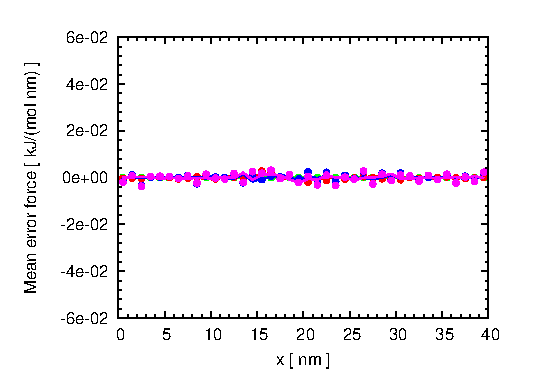
\includegraphics[]{fig/error.one_peak.box40x20x20.b1.000.r3.00.n6.K101x051x051/fig.ana.ewald.meanf.eps}
%   \caption{Example 1: the actual (denoted by dots) and estimated
%     (denoted by straight lines) mean error force of the direct part
%     $\langle\Delta \v F_{\textrm{dir}}\rangle$ (red), reciprocal
%     part of Ewald summation $\langle\Delta \v F_{\textrm{rec}}p\rangle$ (green) and the reciprocal part of the analytical
%     differentiation $\langle\Delta \v
%     F^{\textrm{ana}}_{\textrm{rec}}\rangle$ (blue). The total
%     mean error force of analytical differentiation $\langle\Delta \v
%     F^{\textrm{ana}}\rangle$ is given in pink.  Since the charge
%     distribution is uniform on the $y$ and $z$ direction, the $y$ and
%     $z$ dimension of the mean error force is averaged, and the errors
%     are plotted on $x$ direction.  The cut-off in the real space is 3
%     \textsf{nm}, the number of freedom in the reciprocal space is
%     $100\times 50\times 50$, the parameter $\beta$ is $1.0\;
%     \textsf{nm}^{-1}$ and the order of B-spline interpolation used for
%     the analytical differentiation is 6.}
%   \label{fig:meanf1}
% \end{figure}

% Fig.~\ref{fig:meanf1} presents the mean error force of the direct part
% $\langle\Delta \v F_{\textrm{dir}}\rangle$, reciprocal part of Ewald
% summation $\langle\Delta \v F_{\textrm{rec}}\rangle$ and the
% reciprocal part of the analytical differentiation $\langle\Delta \v
% F^{\textrm{ana}}_{\textrm{rec}}\rangle$. The total mean error force of
% analytical differentiation, which is simply $\langle\Delta \v
% F^{\textrm{ana}}\rangle = \langle\Delta \v F_{\textrm{dir}}\rangle +
% \langle\Delta \v F^{\textrm{ana}}_{\textrm{rec}}\rangle$, is also
% given.  The real and estimated mean error forces are denoted by dots
% and straight lines, respectively. All estimates are consistent very
% well with real errors.  Since the system is locally neutral, the first
% order charge distribution $\rho_q$ is naturally zero, therefore, by
% Eqn. \eqref{eqn:tmp10}, \eqref{eqn:tmp18} and \eqref{eqn:ana.meanf}, all
% the mean error forces should varnish. Numerical resutls in
% Fig. \ref{fig:meanf1} verifies with the above discussion.

\begin{figure}
  \centering
  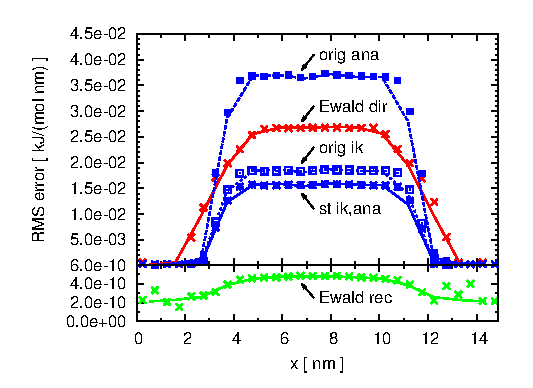
\includegraphics[]{fig.new/fig.rand1.error.eps}
  \caption{
    Example 1: the real RMS errors and the corresponding
    estimates. Different colors denote
    different parts of the Ewald summation. Red: the direct
    part of Ewald summation. Green: the reciprocal
    part of Ewald summation, calculated by truncation.
    ``$\times$'' denotes the real error, and the solid line denotes
    the estimated error.
    Blue: the reciprocal part of Ewald summation, calculated
    by fast algorithms. ``$\blacksquare$'': real error of
    the oringinal analytical
    differentiation. ``$\boxdot$'': real error of the oringinal ik-differentiation.
    ``$\times$'': real error of the staggered mesh analytical differentiation.
    ``$+$'': real error of the staggered mesh ik-differentiation.
    Dashed line: estimated oringinal analytical differentiation.
    Dotted line: estimated oringinal ik-differentiation.
    Solid line: estimated staggered mesh ik-/analytical differentiation.
    The RMS errors are averged over $y$ and $z$ directions, and are
    plotted against $x$ axis.
    The cut-off in the real space is 1.31 \textsf{nm}, the number of
    freedom in the reciprocal space is $120\times 60\times 60$, the
    parameter $\beta$ is $2.5\; \textsf{nm}^{-1}$, and the order of
    B-spline interpolation is 6.
    }
    % Example 1: the actual (denoted by dots) and estimated
    % (denoted by straight lines) RMS force error of the direct part
    % $\sqrt{\langle\vert\Delta \v F_{\textrm{dir}}\vert^2\rangle}$
    % (red), reciprocal part of Ewald summation
    % $\sqrt{\langle\vert\Delta \v F_{\textrm{rec}}\vert^2\rangle}$
    % (green) and the reciprocal part of the analytical differentiation
    % $\sqrt{\langle\vert\Delta \v
    %   F^{\textrm{ana}}_{\textrm{rec}}\vert^2\rangle}$ (blue). The RMS
    % force error of analytical differentiation
    % $\sqrt{\langle\vert\Delta \v F^{\textrm{ana}}\vert^2\rangle}$ is
    % given in pink.  Since the charge distribution is uniform on the
    % $y$ and $z$ direction, the $y$ and $z$ dimension of the mean error
    % force is averaged, and the errors are plotted on $x$ direction.
    % The cut-off in the real space is 3 \textsf{nm}, the number of
    % freedom in the reciprocal space is $100\times 50\times 50$, the
    % parameter $\beta$ is $1.0\; \textsf{nm}^{-1}$ and the order of
    % B-spline interpolation used for the analytical differentiation is
    % 6.}
  \label{fig:error1}
\end{figure}

Fig.~\ref{fig:error1} presents the real RMS error (by points) and the
corresponding error esimates (by lines) of the cut-offed Ewald direct
part, the truncated Ewald reciprocal part, the original ik-/analytical
differentiations and the staggered mesh ik-/analytical
differentiations. All the error estimates are consistent very well
with the real errors, that means the error estimates developed by the
present paper are very sharp.  The parameters of are
chosen to be the same for an easy comparison among these 
SPME branches.  The errors of FFT
based fast Ewald methods are 8 orders of maganitudes large than that of
the truncated Ewald summation.
This supports the argument raised in
Sec.~\ref{sec:error-ik}: the error introduced by truncting the
reciprocal Ewald summation is much smaller than that introduced by
approximating $e^{2\pi i\v m\cdot\v r}$.
The original ik-differentiation is much more accurate than
the original analytical differentiation.
With the staggered mesh,
the error of the analytical differentiation reduces by more than 50\%,
while the accuracy of the ik-differentiation is only marginally
improved.
The errors of the staggered mesh ik- and analytical differentiation
are identical, which supports the theoretical prediction.
The original ik-differentiation uses 4
FFT transforms, and the original analytical differentiation uses
only 2.  Therefore, the staggered mesh analytical differentiation uses
the same amount of FFTs as the original ik-differentiation, and saves
one half than the staggered mesh ik-differentiation.  As mentioned before,
the FFT is a bottleneck of communication on massive parallel
super-computers, so the staggered mesh analytical differentiation
might have advantages on these systems.

% Fig.~\ref{fig:error1} presents the RMS force error of the direct part
% $\sqrt{\langle\vert\Delta \v F_{\textrm{dir}}\vert^2\rangle}$,
% reciprocal part of Ewald summation $\sqrt{\langle\vert\Delta \v
%   F_{\textrm{rec}}\vert^2\rangle}$, the reciprocal part of the
% analytical differentiation $\sqrt{\langle\vert\Delta \v
%   F^{\textrm{ana}}_{\textrm{rec}}\vert^2\rangle}$ and the total
% analytical differentiation force $\sqrt{\langle\vert\Delta \v
%   F^{\textrm{ana}}\vert^2\rangle}$.  The real and estimated mean error
% forces are denoted by dots and straight lines, respectively. All the
% error estimates are overlapping with the real errors, that means the
% error estimates developed by the present paper are very sharp.
% Since all mean error forces varnish, the RMS force errors
% consists of only the homogeneous contribution. 
% In the high charge density region, the error is comparatively larger
% than the low charge density region. For the direct part, the ratio is
% roughly the sqare root of the density ratio. For the reciprocal part
% this ratio is lower. The reciprocal error of the analytical
% differentiation is 4 orders of maganitudes large than that of the
% Ewald summation, which means the Ewald summation is much more precice
% than the fast algorithm based on mesh discretization.


% \begin{figure}
%   \centering
%   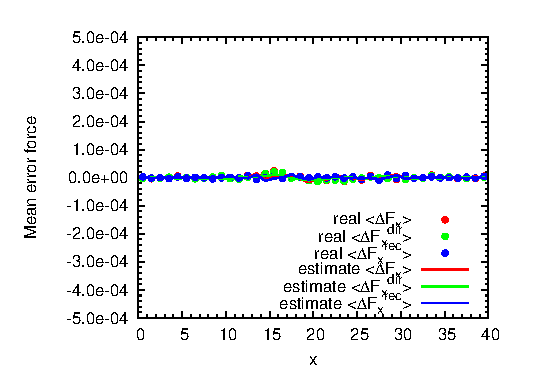
\includegraphics[width=.48\textwidth]{fig/error.one_peak.box40x20x20.b1.000.r3.00.n6.K101x051x051/fig.ik.meanf.eps}
%   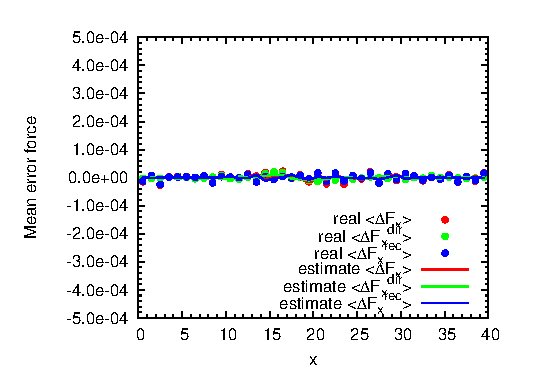
\includegraphics[width=.48\textwidth]{fig/error.one_peak.box40x20x20.b1.000.r3.00.n6.K101x051x051/fig.ana.meanf.eps}
%   \caption{Resulting mean error force}
%   \label{fig:tmp1}
% \end{figure}

% \begin{figure}
%   \centering
%   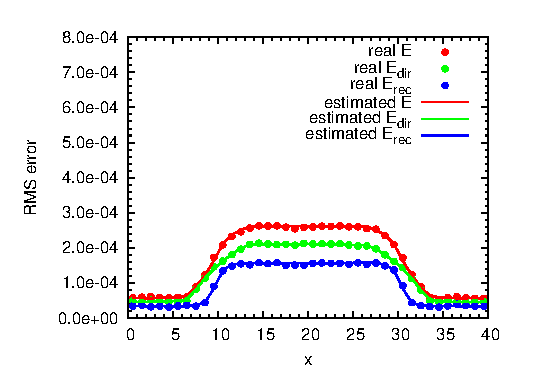
\includegraphics[width=.48\textwidth]{fig/error.one_peak.box40x20x20.b1.000.r3.00.n6.K101x051x051/fig.ik.error.eps}
%   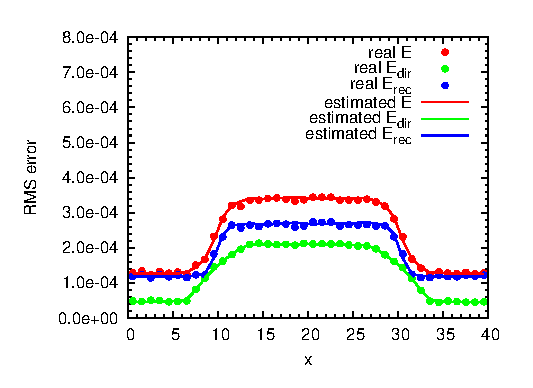
\includegraphics[width=.48\textwidth]{fig/error.one_peak.box40x20x20.b1.000.r3.00.n6.K101x051x051/fig.ana.error.eps}
%   \caption{Resulting RMS errors}
%   \label{fig:tmp2}
% \end{figure}

\subsection{Example 2: seperated positive and negative charge}
\label{sec:example2}

\begin{figure}
  \centering
  % \includegraphics[width=.48\textwidth]{fig.new/rand2/fig.rho.eps}
  \includegraphics[]{fig.new/rand2/fig.rho.eps}
  \caption{Charge distribution of Example 2. The red line
    denotes the positive charge distribution, while the blue line
    denotes the negative charge distribution. Since all distributions
    are uniform on $y$ and $z$ direction, they are plotted as a
    function of $x$.}
  \label{fig:tmp-rho2}
\end{figure}

In this example, the setting is nearly the same as
example 1: 41472 charges are put into a
$14.90\textsf{nm}\times 7.45\textsf{nm}\times 7.45\textsf{nm}$
periodic simulation box. One third of them are carrying negative
charge of $-0.834e$, and the other two thirds are carrying positive
charge of $+0.417e$.  The only difference is that all positive charges
are moved to the region where the density of negative charge is low,
see Fig.~\ref{fig:tmp-rho2}.
In this system, the nagative charges are seperated from their
counter ions, but the whole system is kept neutral. This case rarely
happens in real simulation, but serves as a good test of the error
estimates in extreme situations.

\begin{figure}
  \centering
  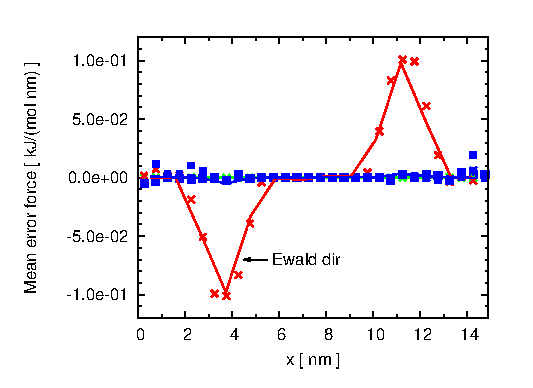
\includegraphics[]{fig.new/fig.rand2.meanf.eps}
  \caption{
    Example 2: the real mean error forces and the corresponding
    estimates. All symbols and working parameters are the same
    as     Fig.~\ref{fig:error1}.
    The reciprocal mean error forces vanish, so the points and lines
    overlap each other. 
    The errors are averged over $y$ and $z$ directions, and are
    plotted against $x$ axis.
    % Red: the direct
    % part of Ewald summation. Green: the reciprocal
    % part of Ewald summation, calculated by truncation.
    % ``$\times$'' denotes the real error, and the solid line denotes
    % the estimated error.
    % Blue: the reciprocal part of Ewald summation, calculated
    % by fast algorithms. ``$\blacksquare$'': real error of
    % the oringinal analytical
    % differentiation. 
    % ``$\times$'': real error of the staggered mesh analytical differentiation.
    % Dashed line: estimated oringinal analytical differentiation.
    % Solid line: estimated staggered mesh ik-/analytical differentiation.
    % The $x$ component of the
    % error forces are averged over $y$ and $z$ directions, and are
    % plotted against $x$ axis.
    % The cut-off in the real space is 1.31 \textsf{nm}, the number of
    % freedom in the reciprocal space is $120\times 60\times 60$, the
    % parameter $\beta$ is $2.5\; \textsf{nm}^{-1}$, and the order of
    % B-spline interpolation is 6.
    }
  \label{fig:meanf2}
\end{figure}


Fig.~\ref{fig:meanf2} shows the real mean error forces (by points) and the
corresponding error esimates (by lines) of cut-offed Ewald direct
part, truncated Ewald reciprocal part, the original
and the staggered mesh analytical differentiation. All
notations in the figure are the same as Example 1.  Although the
charge distribution is not usual in this case, the error estimates are
sharp. The two peaks of the direct mean  error force present at the
positive-negative interface, due to the seperation of the positive
and nagative charges, i.e., a non-vanishing and fast changing first order charge
distribution $\rho_q$.  Similar phenomena were reported by
Ref.~\cite{wang2012}. Surprisingly, 
the reciprocal mean error forces
do not present any singularity, and varnish
all over the simulation region.

\begin{figure}
  \centering
  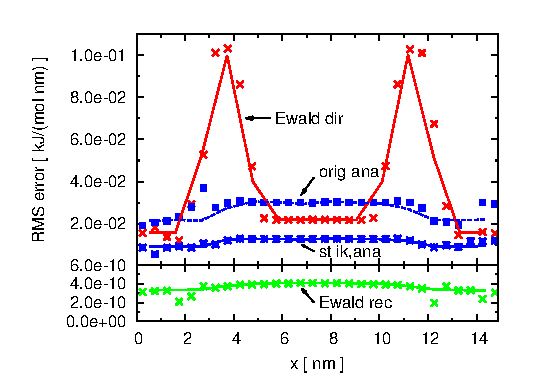
\includegraphics[]{fig.new/fig.rand2.error.eps}
  \caption{
    Example 2: the real RMS error and the corresponding
    estimates.
    The symbols and working parameters used in this figure are the same as
    Fig.~\ref{fig:error1}.
    The real and estimated error of the original ik-differentiation
    are very closed to the staggered mesh Ewald results, so
    they are not shown in this figure for clarity, 
    The errors are averged over $y$ and $z$ directions, and are
    plotted against $x$ axis.
  }
  \label{fig:error2}
\end{figure}

Fig.~\ref{fig:error2} presents the real RMS error of example 2. The
results of the original and staggered mesh ik-differentiation are not
shown, because they are nearly indistinguishable from the staggered
mesh analytical differentiation in this plot.
All the error estimates consist with the real errors.
Steming from the inhomogeneity error,
two peaks of the direct error form at the interfacial
regions, and are much larger than the error in bulk
regions~\cite{wang2012}.
The reciprocal RMS errors only contain homogeneity contributions,
due to the varnished mean error force.
Similar with Example 1, the truncated Ewald
method is much more precise than the fast algorithms, and the
staggered mesh method improves the accuracy of analytical
differentiation by more than 50\%.


% Fig. \ref{fig:error2} shows the RMS errors of Example 2. The
% corresponding error estimates are accurate. In this case the second
% order charge distrubution is a constant, therefore the contribution to
% the error is also a constant. The same as Example 1, the reciprocal
% error of Ewald sum is much smaller than the direct error and the
% reciprocal error of analytical differentiation.  The error peak at the
% positive-negative interface, is only 3 times larger than the error of
% the bulk regions. For the dispersion interaction, the interfacial
% error could be more than one order of maganitude larger than the bulk
% error. That is because the direct interaction converges much faster
% than the dispersion interaciton ($e^{-r^2}$ v.s. $r^{-6}$).

% \begin{figure}
%   \centering
%   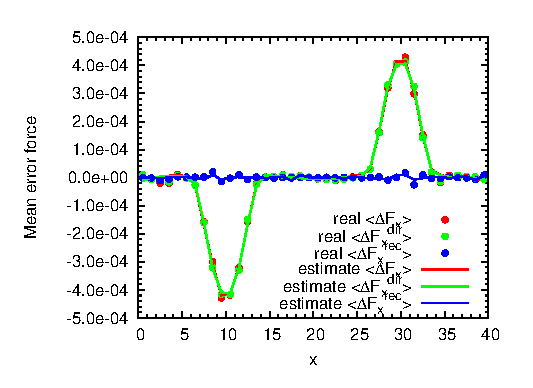
\includegraphics[width=.48\textwidth]{fig/error.two_peaks_sep.box40x20x20.b1.000.r3.00.n6.K101x051x051/fig.ik.meanf.eps}
%   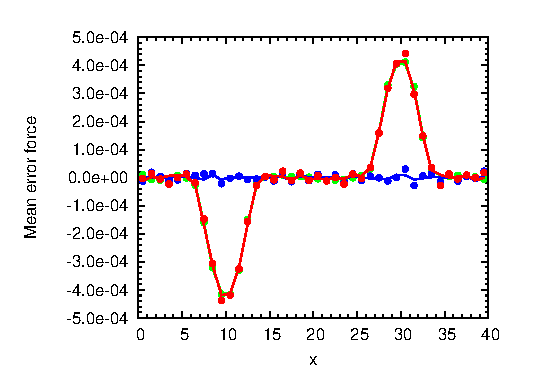
\includegraphics[width=.48\textwidth]{fig/error.two_peaks_sep.box40x20x20.b1.000.r3.00.n6.K101x051x051/fig.ana.meanf.eps}
%   \caption{Resulting mean error force}
%   \label{fig:tmp3}
% \end{figure}

% \begin{figure}
%   \centering
%   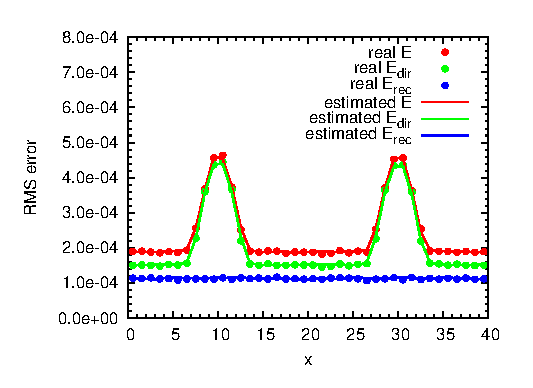
\includegraphics[width=.48\textwidth]{fig/error.two_peaks_sep.box40x20x20.b1.000.r3.00.n6.K101x051x051/fig.ik.error.eps}
%   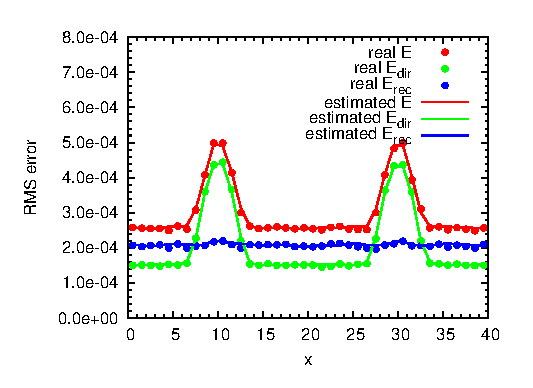
\includegraphics[width=.48\textwidth]{fig/error.two_peaks_sep.box40x20x20.b1.000.r3.00.n6.K101x051x051/fig.ana.error.eps}
%   \caption{Resulting RMS errors}
%   \label{fig:tmp4}
% \end{figure}

\subsection{Example 3: a water system in gas-liquid phase equilibrium}
\label{sec:example3}

This example studies the gas-liquid phase equilibrum of a water
system. The size of the simulation box and number of charges are the
same as Example 1 (Sec.~\ref{sec:example1}): 13824 TIP3P water
molecules~\cite{jorgensen1983comparison} are put into a
$14.90\textsf{nm}\times 7.45\textsf{nm}\times 7.45\textsf{nm}$
periodic simulation box.  The molecules dynamics simulations of this
system is performed by Gromacs 4.5~\cite{hess2008gromacs}.  The system
is coupled to a velocity rescale thermostat~\cite{bussi2007canonical}
at temperature 300~\textsf{K}, and simulated long enough to reach the
equilibrium. After the equibrium,
the water molecules seperate into the liquid and vapor phases.
The number densities of oxygen and hydrogen atoms
are the same as those shown by Fig.~\ref{fig:tmp-rho1}.
50 consequential snapshots of
the system are taken along the MD trajectory
with a time interval of 20~\textsf{ps}.  These
snapshots are used to calculate the real error and the charge densities
for the error estimates.

\begin{figure}
  \centering
  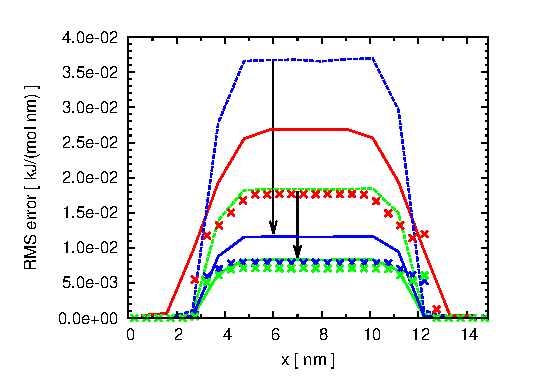
\includegraphics[]{fig.new//fig.water.orig.error.eps}
  \caption{
    Example 3: the real RMS errors and the corresponding
    estimates of original ik- and analytical differentiation.
    The symbols are the same as Fig.~\ref{fig:error1}.
    The cut-off in the real space is 1.35 \textsf{nm}, the number of
    freedom in the reciprocal space is $120\times 60\times 60$, the
    parameter $\beta$ is $2.5\; \textsf{nm}^{-1}$, and the order of
    B-spline interpolation is 6.
  }   
  \label{fig:water-error0}
\end{figure}

\begin{figure}
  \centering
  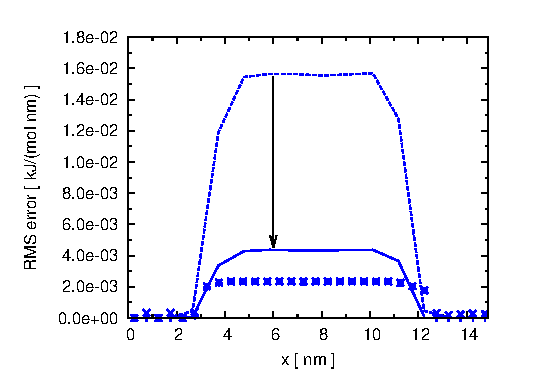
\includegraphics[]{fig.new//fig.water.ana.st.error.eps}
  \caption{
    Example 3: the real RMS errors and the corresponding
    estimates. 
    Red ``$\times$'': the real direct error.
    Red solid line: the estimated direct error.
    Blue ``$\times$'': the real error of the staggered mesh
    analytical differentiation.
    Blue ``$+$'': the real error of the staggered mesh
    ik-differentiation, it is overlapping with the analytical differentiation.
    Blue dashed line: the error estimate of  the staggered mesh Ewald method.
    Blue solid line: the error estimate including the first
    neighbor approximation of the correlation error.
    The RMS errors are averged over $y$ and $z$ directions, and are
    plotted against $x$ axis.
    The cut-off in the real space is 1.35 \textsf{nm}, the number of
    freedom in the reciprocal space is $120\times 60\times 60$, the
    parameter $\beta$ is $2.5\; \textsf{nm}^{-1}$, and the order of
    B-spline interpolation is 6.
  }   
  \label{fig:water-error}
\end{figure}

The real and estimated error of the staggered mesh analytical
differentiation are presented in Fig.~\ref{fig:water-error0}
and Fig.~\ref{fig:water-error}.  In this
case, due to the correlation of the charge positions, the assumption
of independent positions is disturbed, so all estimates overestimate
the real errors.
The quality of the direct
part errors estimates is still good (though not perfect):
the error is overestimated by~50\%.
The ik-differentiation error is overestimated by 2.6 times,
while the analytical differentiation error is overestimated by 4.7 times.
% This indecates that the
% first neigbor correlation is not that important in the error estimate of
% the direct part.
Ref.~\cite{wang2010optimizing} showed that the error estimate
(ik-differentiation in a homogeneous water system) that
is even three times larger than the real error
still works well in the parameter tuning process, so 
error estimate for the ik-differentiation is acceptable, but the error
estimate for the analytical differentiation is problematic.
The error estimate of the staggered mesh analytical differentiation is 6.8 times
larger than the real error,
which means the
positional correlation of charges plays a very important role
in the error estimate. More surprisingly, the correlation
actually greatly reduces the error in force computation.
Currently we have no explaination for this phenomenon.
Anyway, the correlation error $\mathcal
E_{\textrm{correlation}}$ should be included to develop a more accurate error
estimate. 
By including the first neighbor approximation of the
correlation error, the error estimate is imporved greatly
(as indicated by the arrow in Fig.~\ref{fig:water-error}), and is only
twice as large as the real error.
This means among all atomic
correlates (i.e. the chemical bonds, the van der Waals interactions,
the hydrogen bonds, etc.), the first neighbor correlation (chemical bond)
is the most important one, and all
the rest account for the remaining discrepancy between the estimated and real
error.
The error estimate for staggered mesh Ewald is now good enough
for the parameter tuning application.
% In this example, although both error estimates are
% not as sharp as the uncorrelated examples (Example 1 \& 2), they are
% good enough to derive for the parameter
% optimization~\cite{wang2010optimizing}.

\section{Conclusions and remarks}

In this paper, we proposed the error estimate for some state-of-art
algoritms calculating the long-range electrostatic interaction
in a molecular system. They were the Ewald summation, the smooth
particle mesh Ewald (SPME, both ik- and analytical differentiation)
and staggered mesh Ewald (both ik- and analytical differentiation).
Unlike previous error estimates, the new error estimates were
developed for inhomogeneous systems, and did not assume
the uniformity of charge distribution, which is a too strong assumption
for most real molecular simulations.
Moreover, for the pairwise error force, we developed the
first neighbor approximation of the correlation error, which greatly
improved the qulity of the error estimate in the water system.
% was shown to be playing a very important role in an inhomogeneous
% water system.

Some minor contributions of the present work are:
\begin{itemize}
\item In a locally neutral charge system, the inhomogeneity
  error was proved to vanish. Therefore, the error
  is of good property, and no adaptive method nor
  force correction~\cite{wang2012} is necessary. Fortunately, most
  real molecular systems are locally neutral.
\item We explicitly gave the expression of the self-interaction term
  in the analytical differentiation, which was proved to dominant the
  force error in low density systems~\cite{cerutti2009staggered}.  The
  expression helped removing the self-interaction at a very low
  computational cost.
\item The error estimate showed that the Staggered mesh Ewald
  (both ik- and analytical differentiation) are always more precise than
  the original SPME.
\item Unlike the original analytical differentiation
  that violates the Newton's third law, the staggered mesh analytical
  differentiation strictly preserves it.
\item We also proved the equivalence of the staggered mesh ik- and analytical
  differentiation, to the leading order of the force error.
  The staggered mesh analytical differentiation requires only one half
  FFTs as the ik-differentiation, so the former may be preferable
  for massive parallel simulation, due to the bottleneck of all-to-all
  communication required by the parallel FFT.
\end{itemize}

The effectivenss of the proposed error estimates was verified by
three numerical tests: two ideal inhomogeneous cases, in which the charges
are randomly distributed,
and one real water system, in which the charges are correlated.
In the ideal cases, the all error estimates are sharp, even in the extreme
case: positive and negative charges are globally seperated. 
In the water system,  all estimates overestimate the real error,
because of the correlation of charges.
The qulitity of  error estimates for the
real space  and the original ik-differentiation is acceptable.
However, the error estimate neglecting the charge correlation
is not applicable  for the staggered mesh Ewald method.
We included the correlation error by the first neighbor approximation,
and the 
the qulity of the
error estimate (of staggered mesh Ewald) was improved greatly.
This indicates among all possible correlations, the first
neighbor correlation is dominant.

This paper only focuses on the accuracy of the
mentioned long-range alrgoritms.
We do not touch the topic of comparing the efficiency of these algoritms.
For a fair comparison, we propose controling a target accuracy,
optimizing working parameters for each algorithm and then comparing
the excution speed.
Such a comparison includes the topic of the hardware architecture,
the communication bandwidth,
the software implementation, the scale of the problem,
the density of the system, etc.. They are far beyond the scope of the current
work, and will be discuss in the following research.




\newpage
\appendix
\section{Error estimate of the Ewald summation}
\label{sec:appendix}



\newpage

\bibliography{ref}{}
\bibliographystyle{unsrt}


\end{document}
